\chapter{Methodology}

\label{chapter4}

In this chapter, we discuss about the techniques and methods used to devise an experiment involving a Pt-Cu bilayer system and subsequently investigate the effect of spin current via SHE.

\section{Experimental plan}

In earlier studies, it has been shown that a pure spin current can be generated and manipulated via a heavy metal through SHE \cite{hirsch1999spin,sinova2004universal,zhang2000spin}. The detection of this spin current can only be done via conversion into charge current (which is measurable) using ISHE. This generally involves a ferromagnetic layer or a magneto-optical method \cite{kimura2007room,li2019spin,stamm2017magneto}.

In our study, we intend to explore the detection of spin current in a NM/HM bilayer system without a magnetic layer.

\section{Preparation of sample}

We prepare a trilayer system, using copper (Cu) as the NM and platinum (Pt) as the HM. Here, we sandwich a layer of Cu between two layers of Pt. This is depicted in \cref{layers}.

\begin{figure}
    \centering
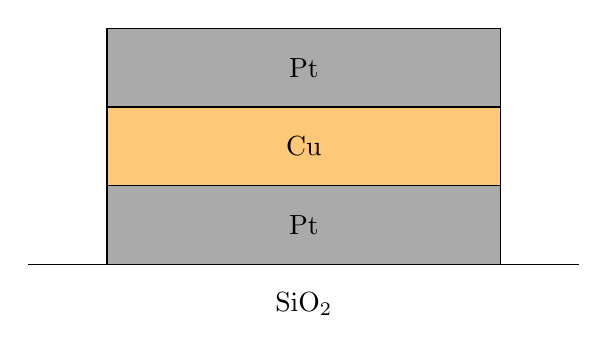
\begin{tikzpicture}
    \draw [fill={rgb:black,1;white,2}] (0,0) rectangle (5,3);
    \node at (2.5,2.5) {Pt};
    \draw [fill={rgb:orange,1;yellow,2;pink,5}] (0,0) rectangle (5,2);
    \node at (2.5,1.5) {Cu};
    \draw [fill={rgb:black,1;white,2}] (0,0) rectangle (5,1);
    \node at (2.5,0.5) {Pt};
    \draw (-1,0) -- (6,0);
    \node at (2.5,-0.5) {SiO$_2$};
\end{tikzpicture}
    \caption{Schematic diagram of trilayer sample}
    \label{layers}
\end{figure}
